\documentclass[border=3pt,tikz]{standalone}
% Shared look for every TikZ figure in these notes.
% Included by each standalone figure file; also keeps the figures consistent
% with the colours used in the PDF and on the website.

\usepackage{tikz}
\usepackage{pgfplots}
\pgfplotsset{compat=1.18}
\usetikzlibrary{arrows.meta, decorations.markings, decorations.pathmorphing,
                patterns, calc, positioning}
\usepackage{amsmath}

% Series colours are the three validated categorical slots also used by the
% interactive widgets, so a path drawn in the printed notes and the same path on
% the website are the same colour. They clear the colour-vision-deficiency and
% contrast checks as a set; every path is direct-labelled as well, so colour is
% never the only thing carrying identity.
\definecolor{duPurple}{HTML}{68246D}
\definecolor{duBlue}{HTML}{2A78D6}
\definecolor{duRed}{HTML}{EB6834}
\definecolor{duGreen}{HTML}{1BAF7A}
\definecolor{duGrey}{HTML}{6B6B6B}

\tikzset{
  axisline/.style   = {-{Stealth[length=3mm]}, line width=0.7pt, black},
  path1/.style      = {duBlue,   line width=1.1pt},
  path2/.style      = {duRed,    line width=1.1pt},
  path3/.style      = {duGreen,  line width=1.1pt},
  statedot/.style   = {circle, fill=black, inner sep=1.4pt},
  arrowhead/.style  = {decoration={markings,
                        mark=at position #1 with {\arrow{Stealth[length=2.6mm]}}},
                       postaction={decorate}},
  lbl/.style        = {font=\small},
  slbl/.style       = {font=\footnotesize, duGrey},
  workfill/.style   = {duPurple, opacity=0.16},
}

% Corollary 3: three reversible engines between the same two reservoirs
\begin{document}
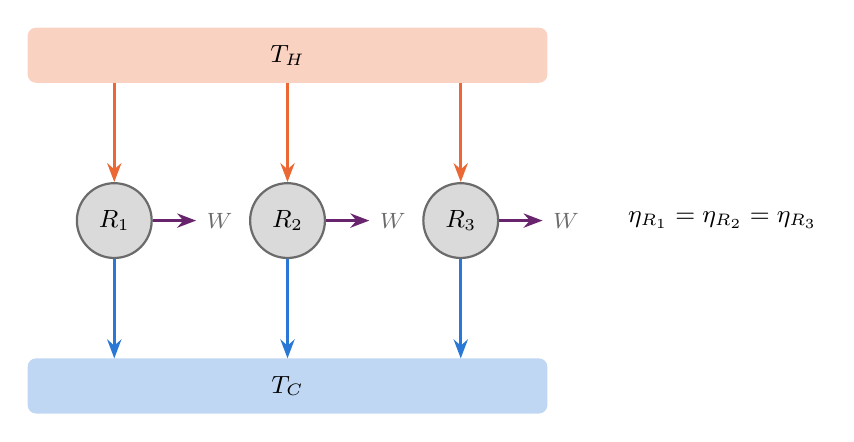
\begin{tikzpicture}[x=1cm,y=1cm,
    res/.style={draw=none, rounded corners=3pt, minimum width=6.6cm, minimum height=0.7cm, font=\small\bfseries},
    eng/.style={circle, draw=duGrey, fill=duGrey!25, line width=0.8pt, minimum size=0.95cm, font=\small},
    flow/.style={-{Stealth[length=2.4mm]}, line width=1.1pt}]
  \node[res, fill=duRed!30] at (0,2.1) {$T_H$};
  \node[res, fill=duBlue!30] at (0,-2.1) {$T_C$};
  \foreach \x/\n in {-2.2/1, 0/2, 2.2/3} {
    \node[eng] (E\n) at (\x,0) {$R_\n$};
    \draw[flow, duRed] (\x,1.75) -- (E\n.north);
    \draw[flow, duBlue] (E\n.south) -- (\x,-1.75);
    \draw[flow, duPurple] (E\n.east) -- ++(0.55,0) node[right, slbl] {$W$};
  }
  \node[lbl, right] at (4.2,0) {$\eta_{R_1} = \eta_{R_2} = \eta_{R_3}$};
\end{tikzpicture}
\end{document}
